\documentclass[main.tex]{subfiles}
\begin{document}
\section{Question 1}
A pipe setup is given below that involves three processes. P is the parent
process, and C1 and C2 are child processes, spawned from P. The pipes are named
p1, p2, p3, and p4. Write a program that establishes the necessary pipe
connections, setups, and carries out the reading/writing of the text in the
indicated directions. (see figure in pdf)

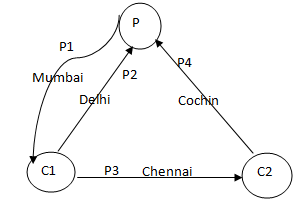
\includegraphics[width=0.8\textwidth]{figures/q1.png}

\lstinputlisting[style=codeStyleC]{listings/1.c}
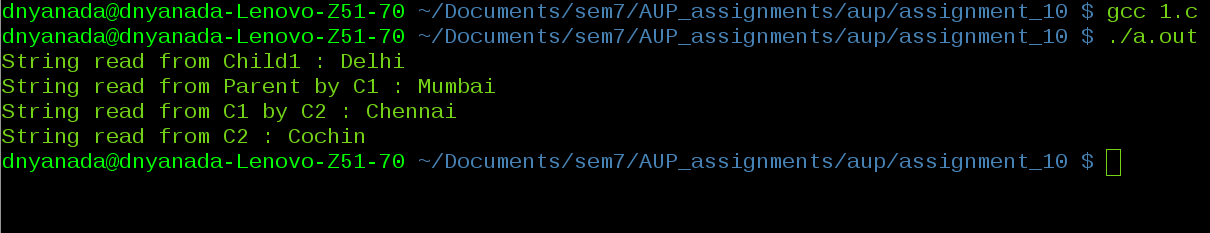
\includegraphics[width=\textwidth]{figures/1_output.png}
\end{document}
